\textbf{\Large{Inleiding}}\\\\
Gezichtsherkenning is een veel voorkomende methode om aan biometrische authenticatie te doen. Het is een onmisbaar kenmerk voor de huidige smartphone of laptop. Het vergemakkelijkt het ontgrendelen van systemen omdat men geen wachtwoord moet onthouden en het razend snel gaat.

Echter zijn gebruikers bezorgd over de betrouwbaarheid van hoe met deze biometrische data wordt omgegaan. Huidige implementaties zorgen ervoor dat de biometrische data (afbeelding van het gezicht van de gebruiker) het toestel van de gebruiker nooit verlaat. Dit betekent dat de berekeningen volledig lokaal en offline gebeuren. Hierdoor kan de privacy van de gebruiker niet geschonden worden. Echter zijn er enkele nadelen die men niet heeft wanneer de berekeningen uitbesteedt worden aan een derde partij via een gedistribueerd  systeem. Indien er kleine aanpassingen of fouten hersteld moeten worden gaat dit veel sneller en effici\"enter als men \'e\'en enkele gecentraliseerde instantie moeten updaten, in plaats van een groot aantal toestellen van gebruikers.

\begin{figure}[H]
  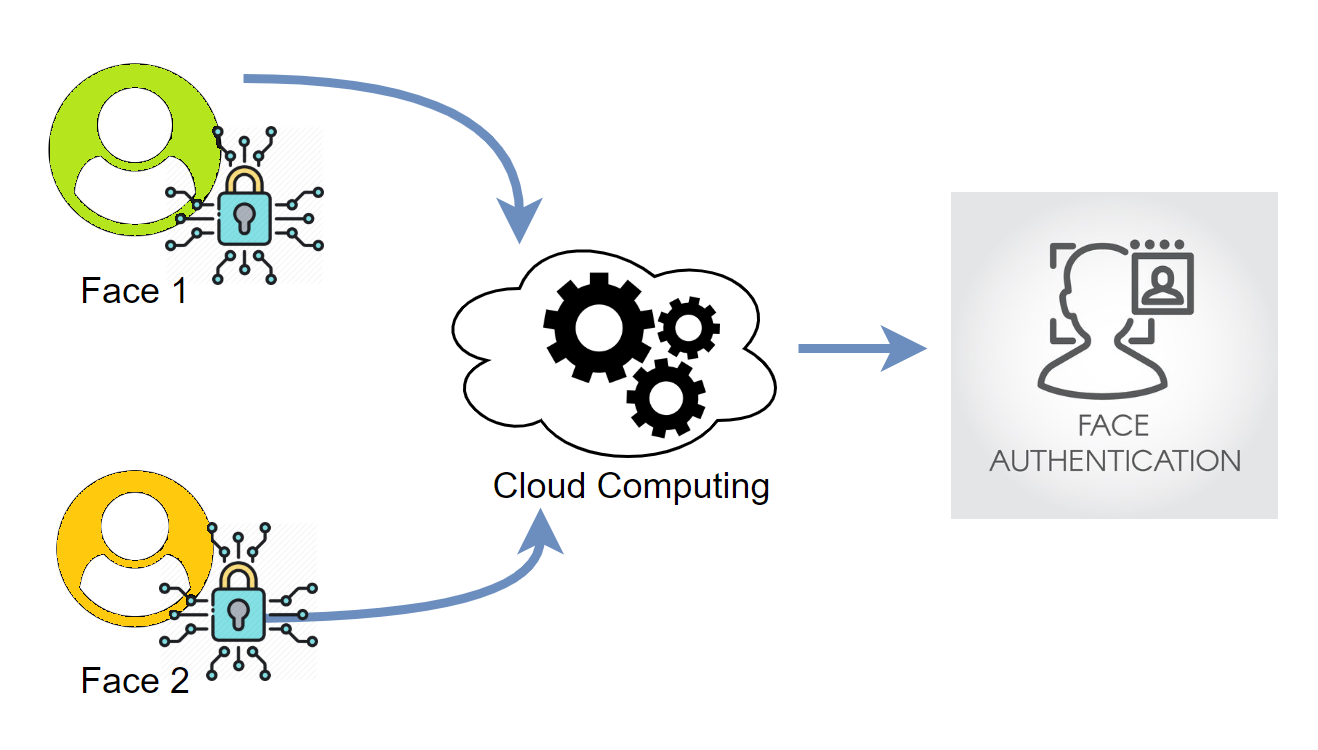
\includegraphics[scale=0.4]{fig/intro_overview.png}
  \centering
  \caption{De gezichten worden ge\"encrypteerd  en op deze ge\"encrypteerde data wordt het gezichtsherkenningsalgoritme uitgevoerd.}
  \label{fig:dutch_intro_overview}
\end{figure}

We zijn op zoek naar een manier om de data van de gebruiker te encrypteren op een manier waardoor men nog steeds een gezichtsherkenningsalgoritme op deze ge\"encrypteerde data kunnen laten uitvoeren (figuur \ref{fig:dutch_intro_overview}). De derde partij die dit algoritme uitvoert zal niet in staat zijn om de data te kunnen decrypteren om de afbeelding van het gezicht van de gebruiker te kunnen lezen.\\

We stellen volgende hypotheses op:

\begin{itemize}
  \item Hoe kunnen we op een privacy behoudende wijze, een gezichtsherkenningsalgoritme gebaseerd op Deep Learning, laten uitvoeren op ge\"encrypteerde data?
  \item Hoe kunnen we dit privacy behoudende algoritme optimaliseren om het effici\"enter uit te voeren?
\end{itemize}

In de loop van de thesis zullen we een antwoord proberen te vinden op beide hypotheses.\\\\

\textbf{\Large{Literatuurstudie}}\\\\
Machine learning is een technologie die gebruikt wordt in computer visie om objecten te detecteren en te herkennen. Een state of the art gezichtsherkenningsalgoritme maakt gebruik van Deep Learning een tak van Machine Learning. Het onderscheidt zich van klassieke neurale netwerken, door de grote hoeveelheid lagen die het netwerk telt. Meestal gaat dit gepaard met een hogere accuraatheid ten koste van een hogere complexiteit.

Een convolutioneel neuraal netwerk (CNN) is een speciaal type neuraal netwerk dat naast het klassieke multi layer perceptron deel een convolutioneel deel bevat. Een convolutioneel neuraal netwerk heeft als kenmerk dat het de spatiale eigenschappen van pixels behoudt. Naburige pixels hebben veel meer invloed op elkaar dan globale pixels. Dit is natuurlijk interessant voor classificatie of herkenning van objecten in afbeeldingen. Een volledig convolutioneel neuraal netwerk bestaat uit een samenstelling van volgende lagen:

\begin{itemize}
  \item Convolutie laag
  \item Activatie laag
  \item Pooling laag
  \item Perceptron laag
\end{itemize}

Gezichtsherkenning of gezicht matching is een algoritme dat probeert te bepalen of twee gezichten van dezelfde persoon zijn. Siamese neurale netwerken kunnen voor dit soort taken gebruikt worden. Een siamees neuraal netwerk bestaat uit twee identieke convolutionele neurale netwerken (met zelfde parameters). Het algoritme krijgt twee afbeeldingen als input. Een voor elk convolutioneel neuraal netwerk van het siamees neuraal netwerk. De output bestaat uit twee vectoren. De afstand tussen deze twee vectoren bepaalt de kans dat de twee afbeeldingen gezichten bevatten van dezelfde persoon. Als de afstand groot is zijn de gezichten verschillend. Als de afstand klein is behoren de gezichten tot dezelfde persoon (figuur \ref{fig:dutch_siamese}).

\begin{figure}[H]
  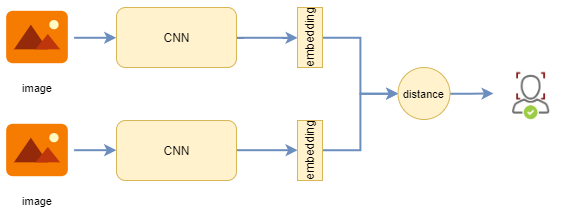
\includegraphics[width=\linewidth]{fig/siamese.png}
  \caption{Siamees neuraal netwerk bestaande uit 2 identieke convolutionele neurale netwerken}
  \label{fig:dutch_siamese}
\end{figure}

Het voordeel van gebruik te maken van siamese neurale netwerken is dat het niet uitmaakt of een nieuw gezicht herkend moet worden. Het netwerk moet niet opnieuw getrained worden.\\

Secure multiparty computation is een protocol dat als doel heeft om verschillende partijen samen methodes te laten berekenen over een aantal inputs op een manier zodat deze inputs priv\'e blijven.

Dit protocol werkt in 3 stappen. Allereerst moet men de inputs encrypteren. Dit gebeurt aan de hand van Shamir's secret sharing schema. Een geheim wordt opgesplitst in verschillende delen, deze delen worden ook shares genoemd. Elk uniek deel wordt aan deelnemer gegeven. Om het geheim te decoderen heb je een minimum aantal shares nodig, de threshold.

De tweede stap is de computatie op deze shares. Men kan een groot aantal operaties doen op de geheime input. Zoals sommatie ($+$) en multiplicatie ($\times$) maar ook relationele operatoren ($\geq$, $=$, ...). Sommige operaties zijn complexer dan andere en vragen dus meer tijd.

De laatste stap is de reconstructie van de shares (dit wordt ook wel decryptie genoemd). Elke partij zendt zijn unieke share uit. Elke deelnemer die een aantal shares heeft groter dan de threshold $t$, kan via Lagrange interpolatie de geheime output decoderen. De geheime input blijft veilig en ge\"encrypteerd en enkel indien $t+1$ corrupte partijen samenwerken, kan de geheime input publiek gemaakt worden. Om dit probleem te voorkomen houden we de threshold $t$ zo hoog mogelijk.

\begin{figure}[H]
  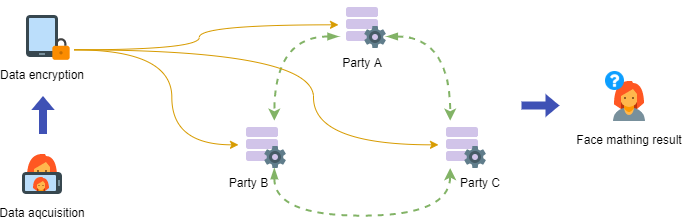
\includegraphics[width=\linewidth]{fig/workflow.png}
  \caption{Workflow van het veilige gezichtsherkenningsalgoritme.}
  \label{fig:dutch_workflow}
\end{figure}

Als men de correct operaties in de correcte volgorde zet zodat men het gezichtsherkenningsalgoritme veilig maakt met secure multiparty computation. Kunnen we de aparte pixels van een afbeelding encrypteren (dit heeft hetzelfde effect als heel de afbeelding encrypteren) met het Shamir secret sharing. Deze shares moeten dan dienen als input van de set van operaties. De output shares kunnen dan worden gereconstrueerd om de output van het gezichtsherkenningsalgoritme te weten te komen (figuur \ref{fig:dutch_workflow}).

Concreet voldoet dit veilige gezichtsherkenningsalgoritme aan twee eisen. De computatie wordt uitbesteedt en de biometrische data van de gebruiker blijft priv\'e.\\\\

\textbf{\Large{Implementatie}}\\\\
In onze praktische implementatie gebruiken we 3 verschillende partijen. We maken gebruik van Docker Desktop om de verschillende partijen te virtualiseren als ge\"isoleerde instanties. Deze kunnen enkel met elkaar communiceren via HTTP. Om de geheime input shares naar de 3 servers te versturen en om deze op te slaan gebruiken we de MongoDB databank. Vervolgens maken we gebruik van 2 belangerijke python packages; Pytorch en MPyC. Pytorch is een library die veel gebruikt wordt door Machine Learning experts. Men kan er snel complexe neurale netwerken mee ontwikkelen en de operaties zijn extreem effici\"ent. Met deze library hebben we een normaal siamees neuraal netwerk gebouwd voor gezichtsherkenning.

MPyC is het framework dat al enkele van de standaard secure multiparty computation operaties ($+$, $-$, $\times$, ...) heeft gedefini\"eerd. We maken hiervan gebruik om complexere operaties zoals ReLU (Rectified Linear Unit), max pooling en convoluties op te stellen.

Tenslotte stellen we enkele manieren voor om het privacy behoudende gezichtsherkenningsalgoritme te optimaliseren. De meest effici\"ente methode is om convoluties die weinig of niets doen weg te laten. Dit principe heet pruning.\\\\

\textbf{\Large{Resultaten en Conclusie}}\\
We hebben in dit project drie aparte experimenten uitgevoerd. In het eerste experiment proberen we aan de hand van twee convoluties een afbeelding te verscherpen. De convolutiefilters zijn zo ingesteld dat ze horizontale en verticale lijnen uit een afbeelding halen. Deze worden dan vermenigvuldigt met een factor en bij de originele afbeelding toegevoegd. Natuurlijk volledig privacy behoudend. Zowel de input als de parameters van de convolutiefilters blijven geheim. Hierdoor onstaat er een verscherpte afbeelding. De twee convoluties op een zwart-wit afbeelding van 100 bij 100 duren iets langer dan een minuut.

Het tweede experiment omvat het testen van de verschillende operaties die voorkomen in convolutionele neurale netwerken (ReLU, max pooling en convoluties) en het delen en reconstrueren van de shares. Hieruit merken we dat convoluties veel meer tijd nemen dan gedacht en aangezien een convolutioneel neuraal netwerk bestaat uit een groot aantal convoluties is dit niet positief.

In ons laatste experiment proberen we alle lagen correct achter elkaar te zetten zoals in het normale convolutionele neurale netwerk. Maar deze keer gebruikmakend van de privacy behoudende operaties. In dit experiment stoten we op technische moeilijkheden. Het systeem crashte omdat er niet genoeg geheugen was. We hebben dus enkel de aparte lagen kunnen demonstreren maar het totale netwerk is niet voltooid geraakt.\\

We concluderen hieruit dat het theoretisch zeker mogelijk is om een gezichtsherkenningsalgoritme privacy behoudend te maken. Maar dat we omwille van technische problemen geen praktische oplossing hebben gevonden. Ook willen we mededelen dat dit protocol extreem complex is. En dat \'e\'en enkele inferentie al gauw 5 tot 10 minuten in beslag kan nemen (gebaseerd op de resultaten van het tweede experiment).
